\documentclass[a4paper, 12pt]{article}

\usepackage[english,russian]{babel}
\usepackage[T2A]{fontenc}
\usepackage[utf8]{inputenc}
\usepackage{geometry}
\usepackage{enumitem}
\usepackage{setspace}
\usepackage{amssymb}
\usepackage{graphicx}
\usepackage{wrapfig}
\usepackage{float}
\usepackage{amsmath}
\usepackage{textcomp}
\usepackage{dsfont}

\geometry{top=5mm, left=1cm}
%\setlength{\parindent}{0}
\renewcommand{\arraystretch}{1.2}
\linespread{1}

\begin{document}
    \begin{center}
        \textbf{Сферическая геометрия №4}\\
        Площадь двуугольника, площадь треугольника.
    \end{center}

    \begin{center}
        \textbf{№ 1}
    \end{center}

    Две сферические прямые пересекаются под углом $\frac{\pi}{6}$.
    Найдите чему равны площади каждого двуугольника, образованного этими прямыми, и посчитайте их сумму,
    если радиус сферы $R=12$ см.

    \textbf{Решение}\\

    \begin{center}
        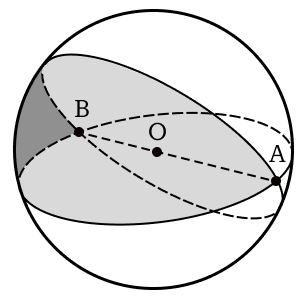
\includegraphics[width=0.2\textwidth]{images/img3}\\
    \end{center}


    1) Пусть $\angle \overline {AB}$ - больший двуугольник, $\overline A, \overline B$ - его углы.
    \[
        \angle A = \frac{\pi}{6}
    \]
    \[ \angle \overline A = \pi - \frac{\pi}{6} = \frac{5\pi}{6}\]

    2)
    \[
        S_{\angle AB} = 2\angle A R ^ 2 = 2 * \frac{\pi}{6} *  144 = 48\pi \text{ см}^2
    \]
    \[
        S_{\angle \overline{AB}} = 2\angle \overline A R ^ 2 = 2 * \frac{5\pi}{6} *  144 = 240\pi \text{ см}^2
    \]

    3)
    \[
        \sum S = 4\pi R ^ 2 = 576 \text{ см}^2
    \]\\

    Ответ: $S_{\angle AB} = 48\pi \text{ см}^2;  S_{\angle \overline{AB}} = 240\pi \text{ см}^2; \sum S = 4\pi R ^ 2 = 576 \text{ см}^2$

    \begin{center}
        \textbf{№ 2}
    \end{center}

    Две сферические прямые пересекаются под углом $\alpha$, третья прямая пересекает две проведенных прямых
    под одинаковыми углами.
    Найдите эти углы, если радиус сферы равен $R$, а площадь сферического треугольника, образованного этими прямыми $S$.

    \textbf{Решение}\\

    \begin{center}
        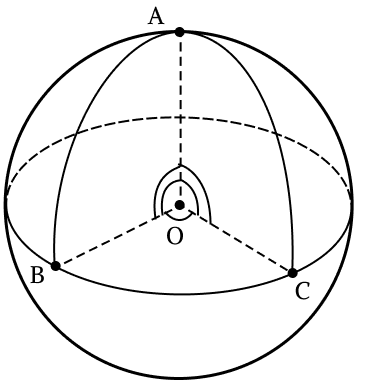
\includegraphics[width=0.2\textwidth]{images/img4}\\
    \end{center}

    1)
    \[
        S_{\triangle ABC} = R^2(\angle A + \angle B + \angle C - \pi) =  R^2(\alpha + 2\angle B - \pi)\rightarrow
        \angle B = \frac{S}{2R^2} - \frac{\alpha- \pi}{2}
    \]

    Ответ: $\frac{S}{2R^2} - \frac{\alpha- \pi}{2} $

    \begin{center}
        \textbf{№ 3}
    \end{center}

    Чему равна площадь сферического треугольника, образованного полюсом и двумя сопряженными с ним точками,
    если сферическое расстояние между этими точками равно $h$, а радиус сферы равен $R$.

    \textbf{Решение}\\

    \begin{center}
        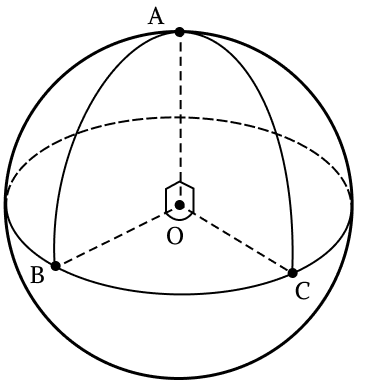
\includegraphics[width=0.2\textwidth]{images/img5}\\
    \end{center}

    1)
    \[
        \angle B = \angle C = \frac{\pi}{2}
    \]
    \[
        \angle A = \frac{h}{R}
    \]

    2) \[
           S_{\triangle ABC} = R^2(\angle A + \angle B + \angle C - \pi) = R^2\frac{h}{R}
    \]

    Ответ: $R^2\frac{h}{R}$

    \begin{center}
        \textbf{№ 4}
    \end{center}

    Дан сферический треугольник с площадью $S$.
    Найдите площадь треугольника с такими же углами на сфере с радиусом в два раза больше.

    \textbf{Решение}\\

    \[
        S_1 = R^2(\angle A + \angle B + \angle C - \pi)
    \]
    \[
        S_2 = (2R)^2(\angle A + \angle B + \angle C - \pi) = 4R^2(\angle A + \angle B + \angle C - \pi) = 4S_1
    \]

    Ответ: $4S$

    \begin{center}
        \textbf{№ 5}
    \end{center}

    Два диаметра, соединяющих пары полюсов пересекаются под углом $\frac{\pi}{6}$,
    чему равны площади двуугольников, образованных их полярами, если радиус сферы равен $19$?

    \textbf{Решение}\\

    1) Как было доказано на занятии 2 в номере 7, угол между диаметрами, соединяющими полюсы,
    равен углу между полярами этих полюсов, тогда на сфере получится два вида двуугольников,
    площадь которых равны:

    \[
        S_1 = 2\frac{\pi}{6} * 19 = \frac{19\pi}{3}
    \]
    \[
        S_2 = 2\frac{5\pi}{6} * 19 = \frac{95\pi}{3}
    \]\\

    Ответ: $\frac{19\pi}{3}$; $\frac{95\pi}{3}$

    \begin{center}
        \textbf{№ 6}
    \end{center}

    Может ли на сфере быть построен сферический треугольник, все углы которого $90^\circ$.
    Если такой треугольник существует, то найдите его стороны и площадь.

    \textbf{Решение}\\

    \begin{center}
        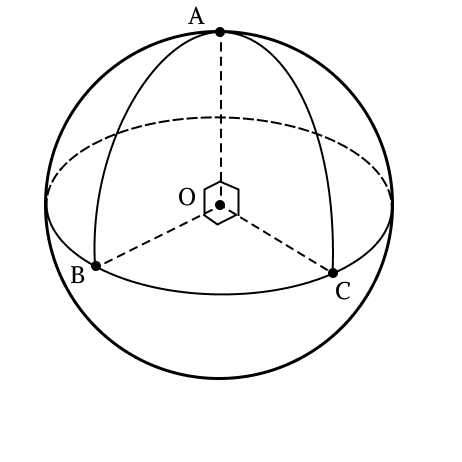
\includegraphics[width=0.2\textwidth]{images/img6}\\
    \end{center}

    Да, такой треугольник образуют три попарно перпендикулярные сферические прямые.

    \[
        \cup AB = \cup AC = \cup BC = \frac{\pi}{2}R
    \]
    \[
        S = R^2\left(\frac{3\pi}{2} - \pi\right) = R^2 * \frac{\pi}{2}
    \]

    Ответ: стороны равны:$\frac{\pi}{2}R$; площадь: $R^2 * \frac{\pi}{2}$

    \begin{center}
        \textbf{№ 7}
    \end{center}

    Пусть стороны сферического треугольника равны $a, b, c$, противолежащие им углы $A, B, C$ соответственно, радиус сферы равен $R$.
    Найдите отношение площадей сферического и планиметрического треугольников, имеющих общие вершины.

     \textbf{Решение}\\

    \begin{center}
        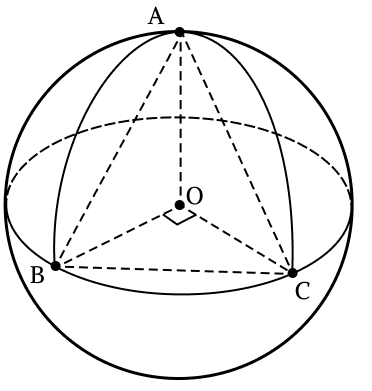
\includegraphics[width=0.2\textwidth]{images/img7}\\
    \end{center}

    1) Найдем углы:
    \[
        \angle BOA = \frac{\cup AB}{R} = \frac{c}{R}
    \]
    \[
        \angle COA = \frac{\cup AC}{R} = \frac{b}{R}
    \]
    \[
        \angle BOC = \frac{\cup BC}{R} = \frac{a}{R}
    \]

    2) Найдем стороны планиметрического треугольника:
    \[
        AB^2 = OB ^ 2 + OA ^ 2 - 2 OB * OA \cos BOA = 2R^2 - 2R^2 \frac{c}{R}
    \]
    \[
        AB = R\sqrt {2-\frac{2c}{r}}
    \]
    \[
        BC =  R\sqrt {2-\frac{2a}{r}}
    \]
    \[
        AC =  R\sqrt {2-\frac{2b}{r}}
    \]

    Площадь сферического треугольника:
    \[
        S_1 = R^2(A +B +C - \pi)
    \]

    Площадь планиметрического треугольника:
    \[
        p = \frac{R\sqrt {2-\frac{2a}{r}} + R\sqrt {2-\frac{2b}{r}} + R\sqrt {2-\frac{2c}{r}}}{2} =
        R\frac{\sqrt {2-\frac{2a}{r}} + \sqrt {2-\frac{2b}{r}} + \sqrt {2-\frac{2c}{r}}}{2} =
    \]
    \[
        S_2 = \sqrt{p\left(p- R\sqrt {2-\frac{2c}{r}}\right)\left(p-R\sqrt {2-\frac{2a}{r}}\right)\left(p-R\sqrt {2-\frac{2b}{r}}\right)} =
    \]
    \[
        \frac{R^2}{\sqrt {2}}\sqrt {\left(\sqrt {2-\frac{2a}{r}} + \sqrt {2-\frac{2b}{r}} - \sqrt {2-\frac{2c}{r}}\right)\left(-\sqrt {2-\frac{2a}{r}} + \sqrt {2-\frac{2b}{r}} + \sqrt {2-\frac{2c}{r}}\right)} *
    \]
    \[
        \sqrt{\left(\sqrt {2-\frac{2a}{r}} - \sqrt {2-\frac{2b}{r}} + \sqrt {2-\frac{2c}{r}}\right)}\cdots
    \]
    Ну на формуле Герона можно и остановиться)

    \begin{center}
        \textbf{№ 9}
    \end{center}

    На сфере радиуса $R$ построен сферический треугольник с сторонами $a, b, c$.
    Найдите евклидово расстояние между каждой парой его вершин и радиус описанной окружности
    около планиметрического треугольника, построенного на вершинах сферического.

    \textbf{Решение}\\

    \begin{center}
        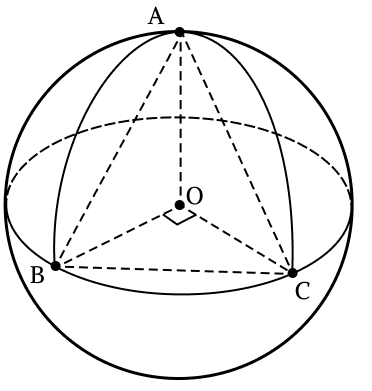
\includegraphics[width=0.2\textwidth]{images/img8}\\
    \end{center}

    1) Найдем стороны планиметрического треугольника:
    \[
        AB = \frac{a}{R}
    \]
    \[
        BC = \frac{b}{R}
    \]
    \[
        AC = \frac{c}{R}
    \]

    2) \[
           R = \frac{AB * BC * AC}{4S}
    \]

    Дальше страшная формула Герона,


    \begin{center}
        \textbf{№ 10}
    \end{center}

    На сфере даны два равнобедренных треугольника, имеющих один равный угол.
    Отношение углов при основании первого треугольника ко второму равно $\delta$.
    Найдите отношение площадей этих треугольников

    \textbf{Решение}\\

    1)
    \[
        S_2 = R ^ 2(A + 2B - \pi)
    \]
    \[
        S_1 = R^2(A + 2B\delta - \pi)
    \]
    2)
    \[
        \frac{S_1}{S_2} = \frac{R ^ 2(A + 2B - \pi)}{R ^ 2(A + 2B\delta - \pi)} = \frac{(A + 2B - \pi)}{(A + 2B\delta - \pi)}
    \]

    Ответ: $\frac{(A + 2B - \pi)}{(A + 2B\delta - \pi)}$

    \begin{center}
        \textbf{№ 11}
    \end{center}

    На сфере дан треугольник, все углы которого равны $90^\circ$.
    На одну из сторон опустили медиану.
    Найдите чему равна площадь получившихся треугольников, если площадь изначального треугольника равна $S$.

     \textbf{Решение}\\

    \begin{center}
        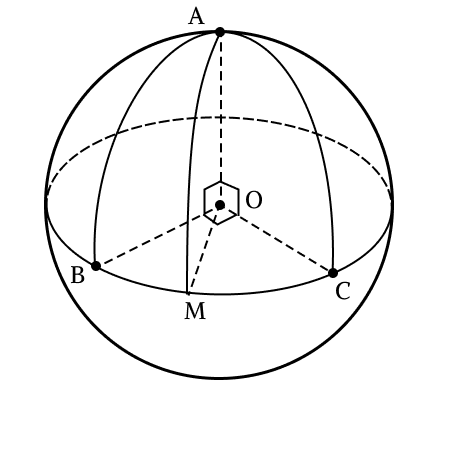
\includegraphics[width=0.2\textwidth]{images/img9}\\
    \end{center}

    1) $AO\bot BOC$ по признаку перпендикулярности прямой и плоскости, тогда $(MOA)\bot(BOC)$ по признаку перпендикулярности
    плоскостей.
    Получаем, что в сферическом треугольнике $\triangle ABM$ $\angle B = \angle M = 90^\circ$

    2) Осталось найти $\angle A$.
    Он равен линейному углу $\angle BOM$
    Так как $\cup BM = \cup MC$, то $\angle BOM \angle MOC = 45^\circ = \frac{\pi}{4}$

    3) Таким образом, искомая площадь равна:
    \[
        S = R^2(\angle BAM + \angle AMB + \angle MBA - \pi) =
        R^2\left(\frac{\pi}{4} + \frac{\pi}{2}+ \frac{\pi}{2} - \pi\right) =
        \frac{R^2\pi}{4}
    \]
    Площадь начального треугольника равна:
    \[
        S_0 = \frac{R^2\pi}{2} \rightarrow S = \frac{S_0}{2}
    \]

    Ответ:$\frac{S_0}{2}$

\end{document}
